\section{Design Technique}
\label{sec:system_design}
The system design is a hardware/software co-design framework for low-power \gls{ml} analytics. This architecture allows design exploration for dedicated hardware in embedded systems. For \gls{ml} compatibility, the proposed framework integrates TensorFlow Lite micro.

\subsection{Base embedded system architecture}
The embedded system architecture consists of a cooperative hardware-software platform. See \Fig{fig:system_architecture}. The embedded \gls{cpu} delegates low-level compute-bound tensor operations to the \glspl{tp}. The \glspl{tp} employ AXI-Lite interface for configuration and AXI-Stream interfaces via \gls{dma} for data movement from off-chip memory. Each \gls{tp} and \gls{dma} pair asserts interrupt flags once its compute job/transaction completes. Interrupt events are handled by the embedded \gls{cpu} to use the results and to start a new compute job/transaction. The hardware architecture can vary its resource utilization by customizing the \glspl{tp} prior to the hardware synthesis.
\begin{figure}[h!]
	\centering
	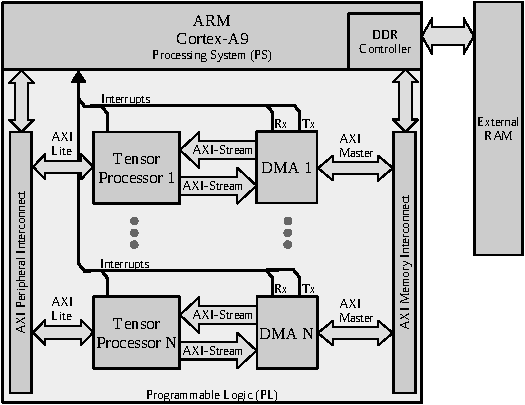
\includegraphics[width=0.5\textwidth]{./chapters/cnn_accelerator/figures/system_design.pdf}
	\caption{Base embedded system architecture.}
	\label{fig:system_architecture}
\end{figure}
\subsection{Tensor processor}
The \gls{tp} is a dedicated hardware module to compute tensor operations. This implements high performance communication with AXI-Stream, direct \gls{cpu} communication with AXI-Lite, and on-chip storage utilizing BRAM. This hardware architecture is implemented with \gls{hls}. The tensor operations are implemented based on the C++ TensorFlow Lite micro kernels. See \fig{fig:accelerator}. This research focuses on the \emph{Conv2D} tensor operation that computes 2D convolution layers.

\begin{figure}[h!]
	\centering
	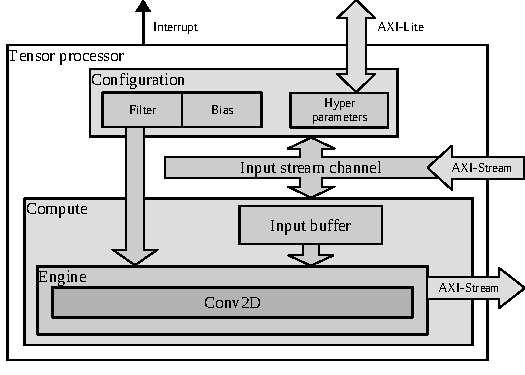
\includegraphics[width=0.5\textwidth]{./chapters/cnn_accelerator/figures/accelerator.pdf}
	\caption{High level hardware architecture of the proposed tensor processor.}
	\label{fig:accelerator}
\end{figure}
\subsubsection{Modes of operation}
The \gls{tp} has two modes of operation: \emph{configuration} and \emph{execution}.
\begin{itemize}
	\item In \emph{configuration} mode, the \gls{tp} receives the hyperparameters of the tensor operation: stride, dilation, padding, offset, activation, depth-multiplier, input shape, filter shape, bias shape, and output shape. Afterwards, in the same data stream, the \gls{tp} receives filter and bias tensors. These are locally stored in BRAM for data re-usage. The filter and bias tensors are transferred using standard \gls{fp} format wrapping the 6-bit \gls{fp} representation, which is extracted by the \gls{tp} for local on-chip storage.
	
	\item In \emph{execution} mode, the \gls{tp} executes the tensor operation according to the hyperparameters given in the configuration mode. During execution, the input and output tensors are moved via \gls{dma}.
\end{itemize}
\subsubsection{Dot-product with hybrid floating-point}
\label{sec:dot_product}
It is implemented the floating-point computation adopting the dot-product with hybrid custom floating-point~\cite{nevarez2021accelerating}. The hardware dot-product is illustrated in \Fig{fig:dot_product} and \Fig{fig:dot_product_loop}(a). This design instantiates a HF6 \gls{mac} with an internal accumulator register of 64-bit fixed-point with 23-bit fraction. During operation, the feature map and filter values are extracted from on-chip memory (BRAM). Both values have to be different than zero to enable the \gls{mac} operation. The result is biased by accumulating a denormalized bias value. Since the bias is stored with 6-bit \gls{fp}, its fractional part has to be aligned with the 23-bit fraction of the accumulator, see \Fig{fig:dot_product_loop}(b). The ReLu activation is applied to the accumulator and its result is normalized to convert it to IEEE 754 standard \gls{fp}, see \Fig{fig:dot_product_loop}(c).

Rather than a parallelized hardware structure, this approach is a pipelined hardware design suitable for resource-limited devices. The latency in clock cycles of this hardware module is defined by \equ{eq:dot_custom_float_latency}, where $N$ is the length for the vector dot-product. This latency equation is obtained from the general pipelined hardware latency formula: $L=\left(N-1\right)II+IL$, where $II$ is the initiation interval, and $IL$ is the iteration latency. Both $II$ and $IL$ are obtained from the \gls{hls} results. Both the exponent and mantissa bit widths of the filter and bias are set to 4-bit exponent and 1-bit mantissa (E4M1), which corresponds to float6 quantization.

\begin{eqnarray} \label{eq:dot_custom_float_latency}
L_{hf}=N+7
\end{eqnarray}

\begin{figure}[h!]
	\centering
	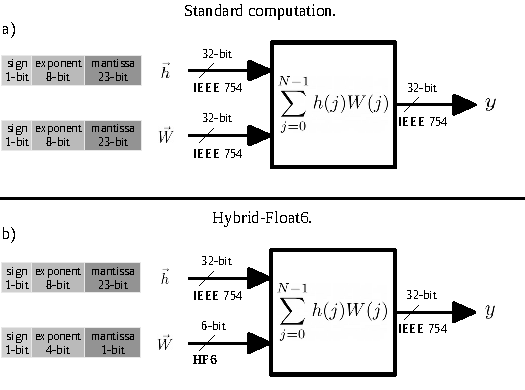
\includegraphics[width=0.5\textwidth]{./chapters/cnn_accelerator/figures/dot-product_unit.pdf}
	\caption{Dot-product hardware module with (a) standard floating-point and (b) Hybrid-Float6.}
	\label{fig:dot_product}
\end{figure}

\begin{figure}[h!]
	\centering
	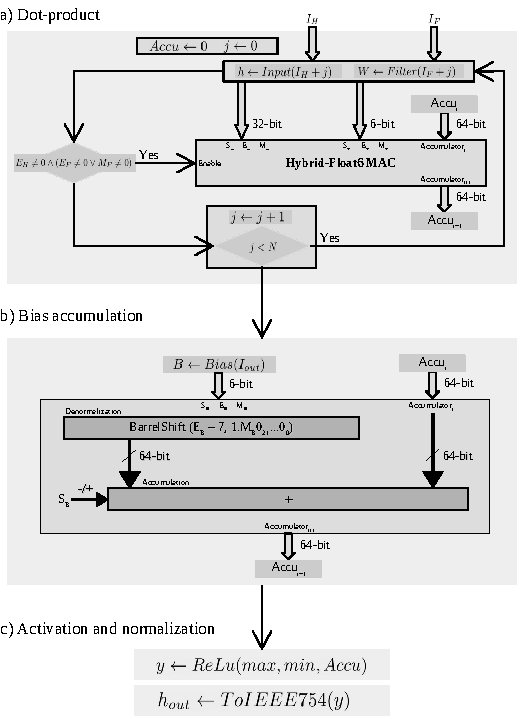
\includegraphics[width=0.5\textwidth]{./chapters/cnn_accelerator/figures/dot_product_hybrid.pdf}
	\caption{(a) Dot-product hardware module with Hybrid-Float6 MAC, (b) bias accumulation, (c) activation and normalization to IEEE754.}
	\label{fig:dot_product_loop}
\end{figure}

\subsubsection{Multiply-Accumulate Unit}
The multiply-accumulate operation calculates the product of two numbers and adds the result to an accumulator. In \gls{fp} arithmetics, the area of a hardware multiplier scales with the bit size of the mantissas. In the case of \gls{hf6}, the 6-bit \gls{fp} representation allows a reduced hardware multiplicator for mantissas. The 1-bit mantissa enables optimized \gls{mac} implementations by reducing the mantissa multiplication to a multiplexed addition, see \fig{fig:multiplier}. This \gls{mac} produces denormalized results, which are accumulated in a fixed-point accumulator. This approach reduces latency, energy consumption, and hardware area/resource utilization.

\begin{figure}[h!]
	\centering
	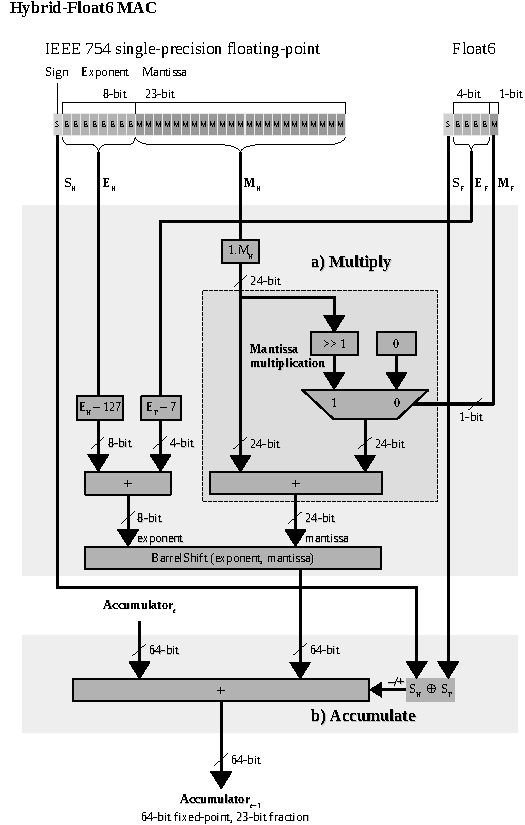
\includegraphics[width=0.5\textwidth]{./chapters/cnn_accelerator/figures/multiplier.pdf}
	\caption{Hybrid-Float6 multiply-accumulate hardware design.}
	\label{fig:multiplier}
\end{figure}

Special cases, such as Infinity and \gls{nan}, are not considered in this design for simplicity, since they are not expected for \gls{cnn} inference. For the subnormal case, the element-wise multiplication is disabled when having a zero entry and approximated when having subnormal mantissa. The feature map values are considered zero when the exponent is zero ($E_H=0$). The filter values are considered zero when both exponent and mantissa are zero ($E_F=0\land M_F=0$). See \Fig{fig:dot_product_loop}(a). In the 6-bit \gls{fp}, the 1-bit mantissa has one subnormal case, which is handled as a normalized case. This exploits the intrinsic error tolerance to reduce the hardware design.

The approximation error is defined by the difference between \Equ{eq:float} and \Equ{eq:float_subnorm} when $E=0$ and $M=2^{-1}$. The result defines the error as $e=2^{-B-1}$. Then, from \Equ{eq:float_bias} with $E_{size}=4$, gives $B=7$. Hence, $e=3.9\mathrm{e}{-3}$. This error is produced when having the subnormal case $E=0$ and $M=2^{-1}$, which corresponds to the value $\pm7.8\mathrm{e}{-3}$ deviated to $\pm1.17\mathrm{e}{-2}$. This approximation leverages the intrinsic error tolerance of \gls{cnn} to reduce hardware resource utilization and energy consumption~\cite{du2014leveraging}.


\subsubsection{On-chip memory utilization}
\label{sec:memory_utilization}
The total on-chip memory utilization on the \gls{tp} is defined by \Equ{eq:tp_memory}, where $TP_B$ and $V_{M}$ represent the tensor buffers required for \emph{Conv} operation and local registers required for the logic, respectively. \Equ{eq:tp_memory_buffer} defines the tensor buffers, where $Input_{M}$ is the \emph{input buffer}, $Filter_{M}$ is the \emph{filter buffer}, $Bias_{M}$ is the \emph{bias buffer}. These on-chip memory buffers are defined in bits. \fig{fig:accelerator_buffers} illustrates the convolution operation utilizing the on-chip memory buffers.
\begin{figure}
	\centering
	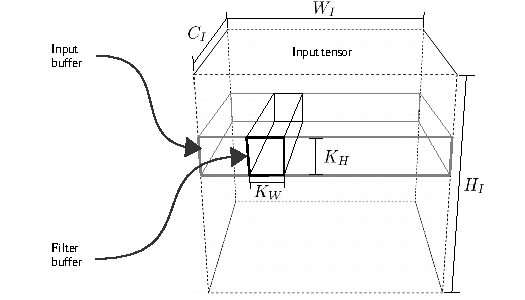
\includegraphics[width=0.5\textwidth]{./chapters/cnn_accelerator/figures/accelerator_buffers.pdf}
	\caption{Design parameters for on-chip memory buffers on the TP.}
	\label{fig:accelerator_buffers}
\end{figure}
\begin{eqnarray} \label{eq:tp_memory}
TP_{M}=TP_B+V_{M}
\end{eqnarray}
\begin{eqnarray} \label{eq:tp_memory_buffer}
TP_{B}=Input_{M}+Filter_{M}+Bias_{M}
\end{eqnarray}

The memory utilization of \emph{input buffer} is defined by \Equ{eq:input_memory}, where $K_{H}$ is the height of the convolution kernel, $W_{I}$ is the width of the input tensor (input feature maps), $C_{I}$ is the number of input channels, and $BitSize_{I}$ is the bit size representation used by the input tensor.
\begin{eqnarray} \label{eq:input_memory}
Input_{M}=K_{H}W_{I}C_{I}BitSize_{I}
\end{eqnarray}

The memory utilization of \emph{filter buffer} is defined by \Equ{eq:filter_memory}, where $K_{W}$ and $K_{H}$ are the width and height of the convolution kernel, respectively; $C_{I}$ and $C_{O}$ are the number of input and output channels, respectively; and $BitSize_{F}$ is the bit size representation used by filter values.
\begin{eqnarray} \label{eq:filter_memory}
Filter_{M}=C_{I}K_{W}K_{H}C_{O}BitSize_{F}
\end{eqnarray}

The memory utilization of \emph{bias buffer} is defined by \Equ{eq:bias_memory}, where $C_{O}$ is the number of output channels, and $BitSize_{B}$ is the bit size representation used by bias values.
\begin{eqnarray} \label{eq:bias_memory}
Bias_{M}=C_{O}BitSize_{B}
\end{eqnarray}

As a design trade-off, \Equ{eq:channel_in_memory} defines the capacity of output channels based on given design parameters. The total on-chip memory $TP_{M}$ determines the \gls{tp} storage capacity.
\begin{eqnarray} \label{eq:channel_in_memory}
C_{O}=\frac{TP_{M}-V_{M}-K_{H}W_{I}C_{I}BitSize_{I}}{C_{I}K_{W}K_{H}BitSize_{F}+BitSize_{B}}
\end{eqnarray}

The floating-point formats implemented in the \gls{tp} are defined by $BitSize_F$, $BitSize_B$ and $BitSize_I$. The HF6 defines 6-bit for $BitSize_F$ and $BitSize_B$, and 32-bit for $BitSize_I$. These are design parameters defined before hardware synthesis. This allows fine control of BRAM utilization, which is suitable for resource-limited devices.

\subsection{Training Method}
The training method consists of two separate stages: (1) training with iterative early stop and (2) quantization-aware training.
 
\subsubsection{Training with Iterative Early Stop}
To achieve better performance on \gls{cnn}-regression models, it implemented a training procedure with iterative early stop cycle. This allows to reach better local minima. This process consists of four steps:

\begin{enumerate}
	\item A model is obtained with an initial training with standard early stop monitoring.
	\item The model is iteratively re-trained with standard early stop. This process iteratively restarts the moving averages of the optimizer to search for better local minima.
	\item In case of a better local minimum, the model is saved and used as a base for subsequent search iterations, otherwise it is a discarded search.
	\item The cyclic process stops automatically with a given number of searches without a better local minimum, this is denoted as stop patience. This allows to set a maximum number of unsuccessful search trials before the stop.
\end{enumerate}

This method is described in \Algo{alg:training}.

\subsubsection{Quantization-Aware Training}
The \gls{qat} method is integrated into the training process, this operates as a callback on each mini-batch update. The quantization is applied on the trainable parameters of convolution layers. This method is implemented on the \gls{ml} framework (TensorFlow/Keras), see \Algo{alg:quantization_integration}.

The quantization method uses rounding strategy to reduce the \gls{fp} representation. This maps the full precision \gls{fp} values to the closest representable 6-bit \gls{fp} values, see \Algo{alg:quantize_training}. This method quantizes the filter and bias tensors of the convolution layers. The exponent bit size plays a more predominant influence on the model accuracy than the mantissa bit size. In \cite{lai2017deep}, Lai \textit{et al.} demonstrated that 4-bit exponent and X-bit mantissa is adequate and consistent across different networks (SqueezeNet, AlexNet, GoogLeNet, VGG-16). In this research, the \gls{fp} representation with 4-bit exponent and 1-bit mantissa is investigated.

\begin{algorithm}[h!]
	\caption{Training with iterative early stop cycle.}
	\label{alg:training}
	\begin{algorithmic}
		\SetAlgoLined
		\renewcommand{\algorithmicrequire}{\textbf{input:}}
		\renewcommand{\algorithmicensure}{\textbf{output:}}
		\REQUIRE $MODEL$ as the input model.
		\REQUIRE $D_{train}$ as the training data set.
		\REQUIRE $D_{val}$ as the validation data set.
		\REQUIRE $N_{I}$ as the stop patience for iterative training cycle.
		\REQUIRE $N_{E}$ as the early stop patience (epochs) for training.
		\REQUIRE $B_{size}$ as the mini-batch size.
		\ENSURE $MODEL$ as the full-precision output model.
		\STATE $Train(MODEL, D_{train}, D_{val}, N_{E}, B_{size})$
		\STATE $mse_i \gets Evaluate(MODEL, D_{val})$ // Benchmark
		\STATE $n_I \gets 0$
		\WHILE {$n_I<N_I$}
		\STATE // Iterative early stop cycle
		\STATE $Train(MODEL, D_{train}, D_{val}, N_{E}, B_{size})$
		\STATE $mse_v \gets Evaluate(MODEL, D_{val})$
		\IF{$mse_v < mse_i$}
			\STATE $Update(MODEL)$
			\STATE $mse_i \gets mse_v$
		\ELSE
			\STATE $MODEL  \gets LoadPreviousWeights()$
			\STATE $n_I \gets n_I + 1$
		\ENDIF
		\ENDWHILE
	\end{algorithmic}
\end{algorithm}


\begin{algorithm}[h!]
	\caption{OnMiniBatchUpdate\_Callback.}
	\label{alg:quantization_integration}
	\begin{algorithmic}
		\SetAlgoLined
		\renewcommand{\algorithmicrequire}{\textbf{input:}}
		\renewcommand{\algorithmicensure}{\textbf{output:}}
		\REQUIRE $MODEL$ as the full-precision input model.
		\REQUIRE $E_{size}$ as the target exponent bits size.
		\REQUIRE $M_{size}$ as the target mantissa bits size.
		\REQUIRE $D_{train}$ as the training data set.
		\REQUIRE $D_{val}$ as the validation data set.
		\REQUIRE $N_{ep}$ as the number of epochs.
		\REQUIRE $B_{size}$ as the mini-batch size.
		\ENSURE $MODEL$ as the quantized output model.
		\STATE // Quantize
		\STATE $MODEL \gets$ \Algo{alg:quantize_training}$(MODEL,E_{size}, M_{size})$ 
		\IF {$1<epoch$}
		\STATE // Update model after first epoch
		\STATE $mse_v \gets Evaluate(MODEL, D_{val})$
		\IF{$mse_v < mse_i$}
		\STATE $Update(MODEL)$
		\STATE $mse_i \gets mse_v$
		\ENDIF
		\ENDIF
	\end{algorithmic}
\end{algorithm}

\begin{algorithm}[h!]
	\caption{Custom floating-point quantization.}
	\label{alg:quantize_training}
	\begin{algorithmic}
		\SetAlgoLined
		\renewcommand{\algorithmicrequire}{\textbf{input:}}
		\renewcommand{\algorithmicensure}{\textbf{output:}}
		\REQUIRE $MODEL$ as the CNN.
		\REQUIRE $E_{size}$ as the target exponent bit size.
		\REQUIRE $M_{size}$ as the target mantissa bits size.
		\REQUIRE $STDM_{size}$ as the IEEE 754 mantissa bit size.
		\ENSURE $MODEL$ as the quantized CNN.
		\FOR {$layer$ in $MODEL$}
		\IF {$layer$ is $Conv2D$ or $SeparableConv2D$}
		\STATE $filter, bias \gets GetWeights(layer)$
		\FOR {$x$ in $filter$ and $bias$}
			\STATE $sign \gets GetSign(x)$
			\STATE $exp \gets GetExponent(x)$
			\STATE $fullexp \gets 2^{E_{size}-1}-1$ // Get full range value
			\STATE $cman \gets GetCustomMantissa(x, M_{size})$
			\STATE $leftman \gets GetLeftoverMantissa(x, M_{size})$
			\IF {$exp <-fullexp$}
				\STATE$x\gets0$
			\ELSIF{$exp > fullexp$}
				\STATE$x\gets (-1)^{sign}\cdot2^{fullexp}\cdot(1+(1-2^{-M{size}}))$
			\ELSE
				\IF {$2^{STDM_{size}-M_{size}-1}-1<leftman$}
					\STATE $cman \gets cman+1$ // Above halfway
					\IF{$2^{M_{size}}-1<cman$}
					\STATE $cman \gets 0$ // Correct mantissa overflow
					\STATE $exp \gets exp + 1$
					\ENDIF
				\ENDIF
				\STATE // Build custom quantized floating-point value
				\STATE$x\gets (-1)^{sign}\cdot2^{exp}\cdot(1+cman\cdot2^{-M_{size}})$
			\ENDIF
		\ENDFOR
		\STATE $SetWeights(layer, filter, bias)$
		\ENDIF
		\ENDFOR
	\end{algorithmic}
\end{algorithm}
\begin{figure}[t!]
	\centering
	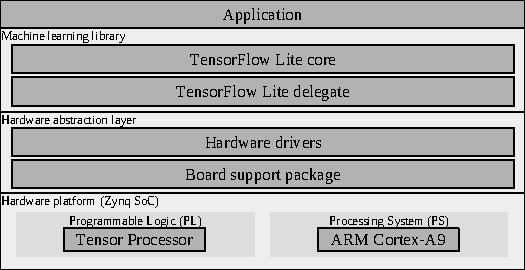
\includegraphics[width=0.5\textwidth]{./chapters/cnn_accelerator/figures/sw_stack.pdf}
	\caption{High level embedded software architecture.}
	\label{fig:sw_stack}
\end{figure}

\begin{figure}[t!]
	\centering
	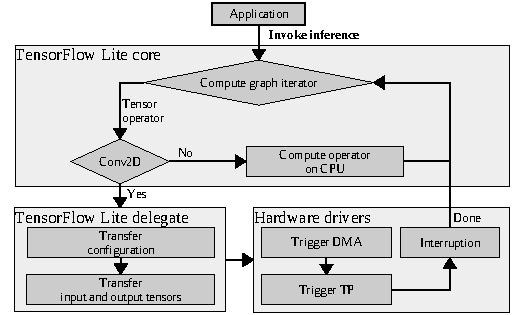
\includegraphics[width=0.5\textwidth]{./chapters/cnn_accelerator/figures/sw_stack_flowchart.pdf}
	\caption{Software flowchart.}
	\label{fig:sw_stack_flowchart}
\end{figure}

\subsection{Embedded software architecture}
The software architecture is a layered object-oriented application framework written in C++, see \fig{fig:sw_stack} and \fig{fig:sw_stack_flowchart}. Description of the software layers is as follows:
\begin{itemize}
	\item \emph{Application}: As the highest level of abstraction, this software layer implements the analytics application, this invokes the \gls{ml} library.
	\item \emph{Machine learning library}: This software layer offers a comprehensive high level \gls{api} for \gls{ml} inference. This layer consist of TensorFlow Lite micro, this is modified to implement the delegate software interfaces for the proposed hardware accelerator.
	\item \emph{Hardware abstraction layer}: This layer consist of the hardware drivers used in the TFLite delegate interfaces. This software layer handles initialization and runtime operation of the \gls{tp} and \gls{dma}.
\end{itemize}